%%%%%%%%%%%%%%%%%%%%%%%%%%%%%%%%%%%%%%%%%
% "ModernCV" CV and Cover Letter
% LaTeX Template
% Version 1.1 (9/12/12)
%
% This template has been downloaded from:
% http://www.LaTeXTemplates.com
%
% Original author:
% Xavier Danaux (xdanaux@gmail.com)
%
% License:
% CC BY-NC-SA 3.0 (http://creativecommons.org/licenses/by-nc-sa/3.0/)
%
% Important note:
% This template requires the moderncv.cls and .sty files to be in the same 
% directory as this .tex file. These files provide the resume style and themes 
% used for structuring the document.
%
%%%%%%%%%%%%%%%%%%%%%%%%%%%%%%%%%%%%%%%%%

%----------------------------------------------------------------------------------------
%	PACKAGES AND OTHER DOCUMENT CONFIGURATIONS
%----------------------------------------------------------------------------------------

\documentclass[11pt,a4paper,sans]{moderncv} % Font sizes: 10, 11, or 12; paper sizes: a4paper, letterpaper, a5paper, legalpaper, executivepaper or landscape; font families: sans or roman

\moderncvstyle{classic} % CV theme - options include: 'casual' (default), 'classic', 'oldstyle' and 'banking'
\moderncvcolor{purple} % CV color - options include: 'blue' (default), 'orange', 'green', 'red', 'purple', 'grey' and 'black'
%\usepackage[italian]{babel}
\usepackage[utf8]{inputenc}
\usepackage{lmodern}
\usepackage{enumitem}
\usepackage{fontawesome5}
\usepackage{ragged2e}
\usepackage{graphicx}
\usepackage{wrapfig}
\usepackage{datatool}

\definecolor{customTeal}{RGB}{0, 128, 128} % RGB for Teal
\definecolor{customTurquoise}{RGB}{64, 224, 208} % RGB for Turquoise
\definecolor{lightGrey}{RGB}{211, 211, 211} % RGB for Light Grey
\definecolor{lightBlue}{HTML}{79B8CF}
\definecolor{blueGray}{HTML}{748FB0}

% Alias
\newcommand{\colorTwo}{blueGray}


% Ensure that what displays C#, grabbing the text gets C-<ascii hex-23 = #>
\newcommand*{\Csh}{C\texttt{\#} }

\newcommand{\repeatsymbol}[2]{%
 \ifnum#1>0%
 	\foreach \n in {1,...,#1}{#2}%
 \fi%
}

\newcommand{\skilllevel}[1]{%
	\repeatsymbol{#1}{\faCircle}\repeatsymbol{\numexpr5-#1\relax}{\faCircle[regular]}%
}

\newcommand{\skl}[1]{%
	\textcolor{white}{#1}% Still presents just the number to document text grab/copy
	\textcolor{\colorTwo}{\skilllevel{#1}}%
}

\usepackage[scale=0.9, top=1cm, bottom=1cm, left=0.7cm, right=0.7cm]{geometry} % Reduce document margins
\setlength{\hintscolumnwidth}{4cm} % Uncomment to change the width of the dates column
%\setlength{\makecvtitlenamewidth}{10cm} % For the 'classic' style, uncomment to adjust the width of the space allocated to your name

%----------------------------------------------------------------------------------------
%	NAME AND CONTACT INFORMATION SECTION
%----------------------------------------------------------------------------------------

\firstname{Francesco} % Your first name
\familyname{Dondi} % Your last name

% All information in this block is optional, comment out any lines you don't need
\title{\small \faIcon{birthday-cake} Born 29/10/1990, Bologna, Italy, \faPassport\  Italian citizen\hfill\ \\
\faGlassCheers Married, no children\hfill\ \\[+0.5em] {\color{black} Latest version of this CV at: \href{https://github.com/Fdondi/cv-latex/blob/main/cv_en.pdf}{github.com/Fdondi/cv-latex/blob/main/cv\_en.pdf}}}
\mobile{+41 76456 50 32\hfill\ }
\email{francesco314@gmail.com\hfill\ }
\social[linkedin]{francesco-dondi\hfill\ }
\social[github]{Fdondi\hfill\ }
\address{\faHouseUser\ Resident Zugerstarsse 66, 8810 Horgen, ZH \hfill\ }
\extrainfo{\\[-0.9em] \faMapMarked \ C permit until 30/09/27 \hfill\ }
\photo[100pt][0pt]{me.jpg} % The first bracket is the picture height, the second is the thickness of the frame around the picture (0pt for no frame)

%----------------------------------------------------------------------------------------

% Store the old definition of \makecvtitle
\let\oldmakecvtitle\makecvtitle

% Redefine \makecvtitle based on the old definition
\renewcommand*{\makecvtitle}{%
  \hfil% push content to the right
  \oldmakecvtitle%
}

\newcommand{\ToolList}[1]{
\hfill
\begin{minipage}[t]{0.15\textwidth}
{\tiny
  \begin{itemize}
    \setlength\itemsep{-0.3em}
    #1
  \end{itemize}
}
\end{minipage}
}

\newcommand{\tsection}[1]{%
	\textcolor{color1}{#1} & \\%
}

\newcommand{\tskl}[2]{%
	#1 & \skl{#2} \\
} 

\begin{document}

\makecvtitle % Print the CV title
\vspace{-12mm}
\begin{minipage}{0.6\linewidth}
\vspace{9mm}
\section{Experience}
\end{minipage}
\begin{minipage}{0.4\linewidth}
\centering
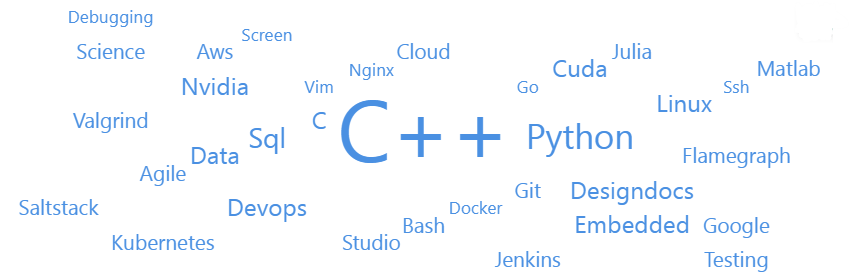
\includegraphics[width=0.99\textwidth]{cloud_long.png}
\vspace{-4mm}
\end{minipage}
\noindent
\begin{minipage}[t]{0.75\linewidth}

\cventry{09/2023 - Current}{Growth time}{}{}{}{
\noindent
\begin{minipage}[t]{0.65\textwidth}
\begin{itemize}
\setlength\itemsep{-0.3em}
\item Continuing German study
\item First personal embedded development project (Arduino)
\item Experimented with LLMs, including 
\begin{itemize}
\setlength\itemsep{-0.5em}
\item prompt engineering: created a CustomGPT to assist with German learning
\item architecture: discovered the details of transformer structure and parameter efficient training
\item learnt to run language models locally, especially Mistral
\end{itemize} 
\end{itemize}
\end{minipage}
}


\cventry{03/2023 - 09/2023 \\ \textbf{DoubleCloud}}{Software Developer}{}{Zürich}{}{
\noindent
\begin{minipage}[t]{0.65\textwidth}
Maintained and developed the infrastructure around managed ClickHouse, in particular:
\begin{itemize}
\setlength\itemsep{-0.3em}
\item Secured metrics server by adding Nginx
\item Improved SaltStack configuration
\item Solved bugs in Telegraf Go plugins
\end{itemize}
\end{minipage}
}

\cventry{10/2022 - 02/2023}{Personal Time}{}{}{}{
\noindent
\begin{minipage}[t]{0.65\textwidth}
\begin{itemize}
\setlength\itemsep{-0.3em}
\item Got married
\item Moved to new house
\item Sailed for a week for the first time
\item Started studying German intensively
\item Got interested in data science
\end{itemize}
\end{minipage}
}

\cventry{06/2021 - 09/2022 \\ \textbf{Firebolt}}{Software Developer}{}{Zürich}{}{
\noindent
\begin{minipage}[t]{0.65\textwidth}
Maintained and developed the SQL optimization engine and testing infrastructure.
\begin{itemize}
\setlength\itemsep{-0.3em}
\item Expanded supported SQL syntax and optimizations
\item reworked the test framework to support new test suite
\item contributed to rewriting to higher standards the optimization engine 
\end{itemize}
\end{minipage}
}

\cventry{08/2020 - 02/2021 \\ \textbf{F-Trust}}{Developer / Analyst}{}{Zug}{}{
\noindent
\begin{minipage}[t]{0.65\textwidth}
\begin{itemize}
\setlength\itemsep{-0.3em}
\item Maintained and developed a Trading Engine (C++)
\item redesigned, implemented and migrated product storage (PostgreSQL)
\item extracted and integrated data from multiple log streams
\item analyzed said data to highlight opportunities for improvement (Julia)
\end{itemize}
\end{minipage}
}

\cventry{10/2017 - 05/2020 \\ \textbf{Google}}{Software Developer}{}{Zürich}{}{
\noindent
\begin{minipage}[t]{0.65\textwidth}
Within Search, productionized an initially experimental tool (C++).
\begin{itemize}
\setlength\itemsep{-0.3em}
\item Improved runtime from days to hours
\item added support for new kinds of data
\item made the results easily visualizable and monitorable
\item made onboarding orders of magnitude faster for most cases
\end{itemize}
\end{minipage}
}

\cventry{04/2016 - 10/2017 \\ \textbf{Ascent Software}}{Software Developer}{}{Luqa, Malta}{}{
\noindent
\begin{minipage}[t]{0.65\textwidth}
Bridging from internal API to new device API for automotive.
\end{minipage}
}


\cventry{04/2015 - 04/2016 \\ \textbf{Rulex Inc.}/\textbf{CNR}}{Junior Developer}{}{Genua, Italy}{}{
\noindent
\begin{minipage}[t]{0.65\textwidth}
Reworked C/MATLAB algorithms for OpenMP/CUDA parallelization
\end{minipage}
}
\end{minipage}
\begin{minipage}[t]{0.25\linewidth}
\vspace{-13mm}
\begin{tabular}{lc}
\tsection{Languages}
English & Fluent \\
Italian & Madrelingua \\
German & B1, B2 geplänt \\
Français & Bon \\
\\
\tsection{Programming}
\tskl{C++}{5}
\tskl{- C++/Abseil}{5}
\tskl{- C++/Boost}{4}
\tskl{SQL}{5}
\tskl{- Clickhouse SQL}{5}
\tskl{- PostgreSQL}{4}
\tskl{Python}{4}
\tskl{Julia}{2}
\tskl{Go}{1}
\tsection{Tools}
\tskl{BASH}{4}
\tskl{Linux}{4}
\tskl{Windows}{3}
\tskl{Visual Studio}{2}
\tskl{AWS storage}{2}
\tskl{Docker}{3}
\tskl{Git}{5}
\tskl{Jenkins CI}{3}
\tskl{SSH}{3}
\tskl{VIM}{3}
\tskl{Valgrind}{3}
\tskl{Flamegraph}{2}
\tskl{Nvidia CUDA}{2}
\tskl{OpenMP}{3}
\tsection{Competences}
\tskl{Testing}{5}
\tskl{Debugging}{4}
\tskl{DevOps}{4}
\tskl{Design Docs}{5}
\tskl{Embedded Dev.}{1}
\tskl{Agile Dev.}{4}
\end{tabular}
\end{minipage}

\pagebreak

\section{Formal education}

\cventry{2023 H1}{\href{https://execed-online.imperial.ac.uk/business-analytics}{Business Analytics: From Data to Decisions}}{Imperial College Business School}{}{}{}
\cventry{2009--2015}{\href{http://www.unipd-scuolagalileiana.it/en/}{Galileian School of Higher Education}}{University of Padua}{University-level enriching program for gifted students}{\textit{98/100}}{}
\cventry{2012--2014}{Master Degree in Mathematics}{University of Padua}{}{\textit{108/110}}{}
\cventry{2009--2012}{Bachelor Degree in Mathematics}{University of Padua}{}{\textit{110/110 cum Laude}}{}
\cventry{2004--2009}{High School - Science Track, added IT, French}{Liceo Fermi}{Bologna}{\textit{100/100 cum Laude}}{}

\section{Continuous Learning}

% <3h: 1-3 lines
% 3-10h: 4-5 lines
% >10h: 6-10 lines

\subsection{Data Science/Analytics}

\cventry{Nov 2023}{Data Fluency: Exploring and Describing Data}{Linkedin}{Barton Poulson}{}{
\begin{minipage}[t]{0.65\textwidth}
how to prepare and adapt data, explore it visually, and use statistical methods to describe it, going in depth on probability and interference. Also touching on data ethics and explainable AI. Thinking with data; preparing data; adapting data; exploring data; describing data; understanding probability and inference.
\end{minipage}
\ToolList{
	\item \faBrain{} Data Science
	\item \faBrain{} Preparing data 
}
\ToolList{
	\item \faBrain{} Exploring data
	\item \faBrain{} Probability
}
}

\cventry{Nov 2023}{Power BI Essential Training}{Linkedin}{Gini von Courter}{3h 45m}{
\begin{minipage}[t]{0.65\textwidth}
Data types in Power BI. Visualizations in Power BI. Outcomes when changes are made within Power BI and Power BI Desktop. Dashboards vs reports within Power BI. User roles within a workspace in Power BI.
Workspaces and tools within the Power BI mobile application.
\end{minipage}
\ToolList{
	\item \faCog{} Microsoft Power BI 
}
\ToolList{	
	\item \faBrain{} Data Visualization
}
}

\cventry{Oct 2023}{Business Intelligence for Consultants}{Linkedin}{Joshua Rischin}{29m}{
\begin{minipage}[t]{0.65\textwidth}
Determine the essentials of business needs. Recognize the fundamentals in reviewing source data. Break down the meaning behind data-driven insights.
\end{minipage}
\ToolList{
	\item \faBrain{} Business Intelligence
}
\ToolList{	
	\item \faBrain{} Data Visualization
}
}

\cventry{Oct 2023}{Data Analytics for Business Professionals}{Linkedin}{John Johnsond}{1h 16m}{
\begin{minipage}[t]{0.65\textwidth}
Real-life analytics in action. Predictive and prescriptive approaches. Formulate and pose your own questions. Collect, clean, and aggregate data from different sources. Identify when data is flawed.
\end{minipage}
\ToolList{
	\item \faCog{} Pandas	
	\item \faCog{} Databases
}
\ToolList{	
	\item \faBrain{} Data Analytics
	\item \faBrain{} Data Visualization
}
}


\cventry{Oct 2023}{Excel: Economic Analysis and Data Analytics}{Linkedin}{Michael McDonald}{2h 17m}{
\begin{minipage}[t]{0.65\textwidth}
Using regression analysis, confidence intervals, and forecasting tools with your company’s key performance indicators (KPIs), building your skill set in data analytics to better meet the needs of your business.
\end{minipage}
\ToolList{
	\item \faCog{} Microsoft Excel	
	\item \faBrain{} Economic Analysis
}
\ToolList{
	\item \faBrain{} Data Analytics
	\item \faBrain{} Data Visualization
}
}

\cventry{Oct 2023}{The Non-Technical Skills of Effective Data Scientists}{Linkedin}{Keith McCormick}{44m}{
\begin{minipage}[t]{0.65\textwidth}
New data scientists must be able to empathize, persuade, and lead others if they want to successfully run projects that produce business transformation.
\end{minipage}
\ToolList{
	\item \faBrain{} Business communication
}
\ToolList{
	\item \faBrain{} Data Science
}
}


\subsection{AI and LLMs}

\subsection{Programming languages}

\cventry{Nov 2023}{\Csh Essential Training 1: Types and Control Flow}{Linkedin}{ Matt Milner}{2h 38m}{
\begin{minipage}[t]{0.65\textwidth}
\Csh in context; .NET, MSIL, and the Base Class Library. Fundamental patterns  of \Csh from control flow to enums and switch matches.
\end{minipage}
\ToolList{
	\item \faPencil*{}\Csh 
}
\ToolList{
	\item \faBrain{} \Csh patterns 
}
}

\cventry{Oct 2023}{Learning MATLAB}{Linkedin}{Steven Moser}{1h 13m}{
\begin{minipage}[t]{0.65\textwidth}
MATLAB tools to model data and hypotheses
\end{minipage}
\ToolList{
	\item \faPencil*{} MATLAB 
}
\ToolList{
	\item \faBrain{} Data Processing 
}
}

\subsection{Embedded development}

\cventry{Nov 2023}{C Programming for Embedded Applications}{Linkedin}{Eduardo Corpeño}{2h 5m}{
\begin{minipage}[t]{0.65\textwidth}
Deliver applications that are small, efficient, and fast for the Internet of Things. Memory, storage, power limitations, and hardware awareness.
\end{minipage}
\ToolList{
	\item \faPencil*{} C Embedded
}
\ToolList{
	\item \faBrain{} Embedded Development 
}
}

\subsection{Cloud and DevOps}

\cventry{Feb 2023}{AWS Certified Solutions Architect - Associate (SAA-C02) Cert Prep: 1 Cloud Services Overview}{Linkedin}{Tom Carpenter}{1h7m}{
\begin{minipage}[t]{0.65\textwidth}
AWS services, security solutions of AWS, AWS regions and availability.
\end{minipage}
\ToolList{
	\item \faCog{} AWS Cloud 
}
\ToolList{
	\item \faBrain{} Cloud Computing 
}
}

\cventry{Jan 2023}{DevOps Foundations: Going Cloud Native}{Linkedin}{Karthik Gaekwad}{45m}{
\begin{minipage}[t]{0.65\textwidth}
The information senior executives —CTOs, vice presidents, and chief architects— need to know to embrace cloud native.
\end{minipage}
\ToolList{
	\item \faBrain{} DevOps 
}
\ToolList{
	\item \faBrain{} Cloud Development 
}
}

\section{Projects}

\subsection{Embedded}

\cventry{Nov 2023}{BTC Arduino monitor}{\href{https://github.com/Fdondi/arduino-btc}{https://github.com/Fdondi/arduino-btc}}{}{}{
\begin{minipage}[t]{0.6\textwidth}
A bot checking Bitcoin prices and blinking a green led if the price is above average, red if below. The speed of blinking depends on the magnitude of the change. 
\end{minipage}
\ToolList{
	\item \faPencil*{} Embedded C++ 
	\item \faCog{} Arduino
	\item \faCog{} Embedded web API 
}
\begin{minipage}[t]{0.2\textwidth}
\vspace{-8mm}
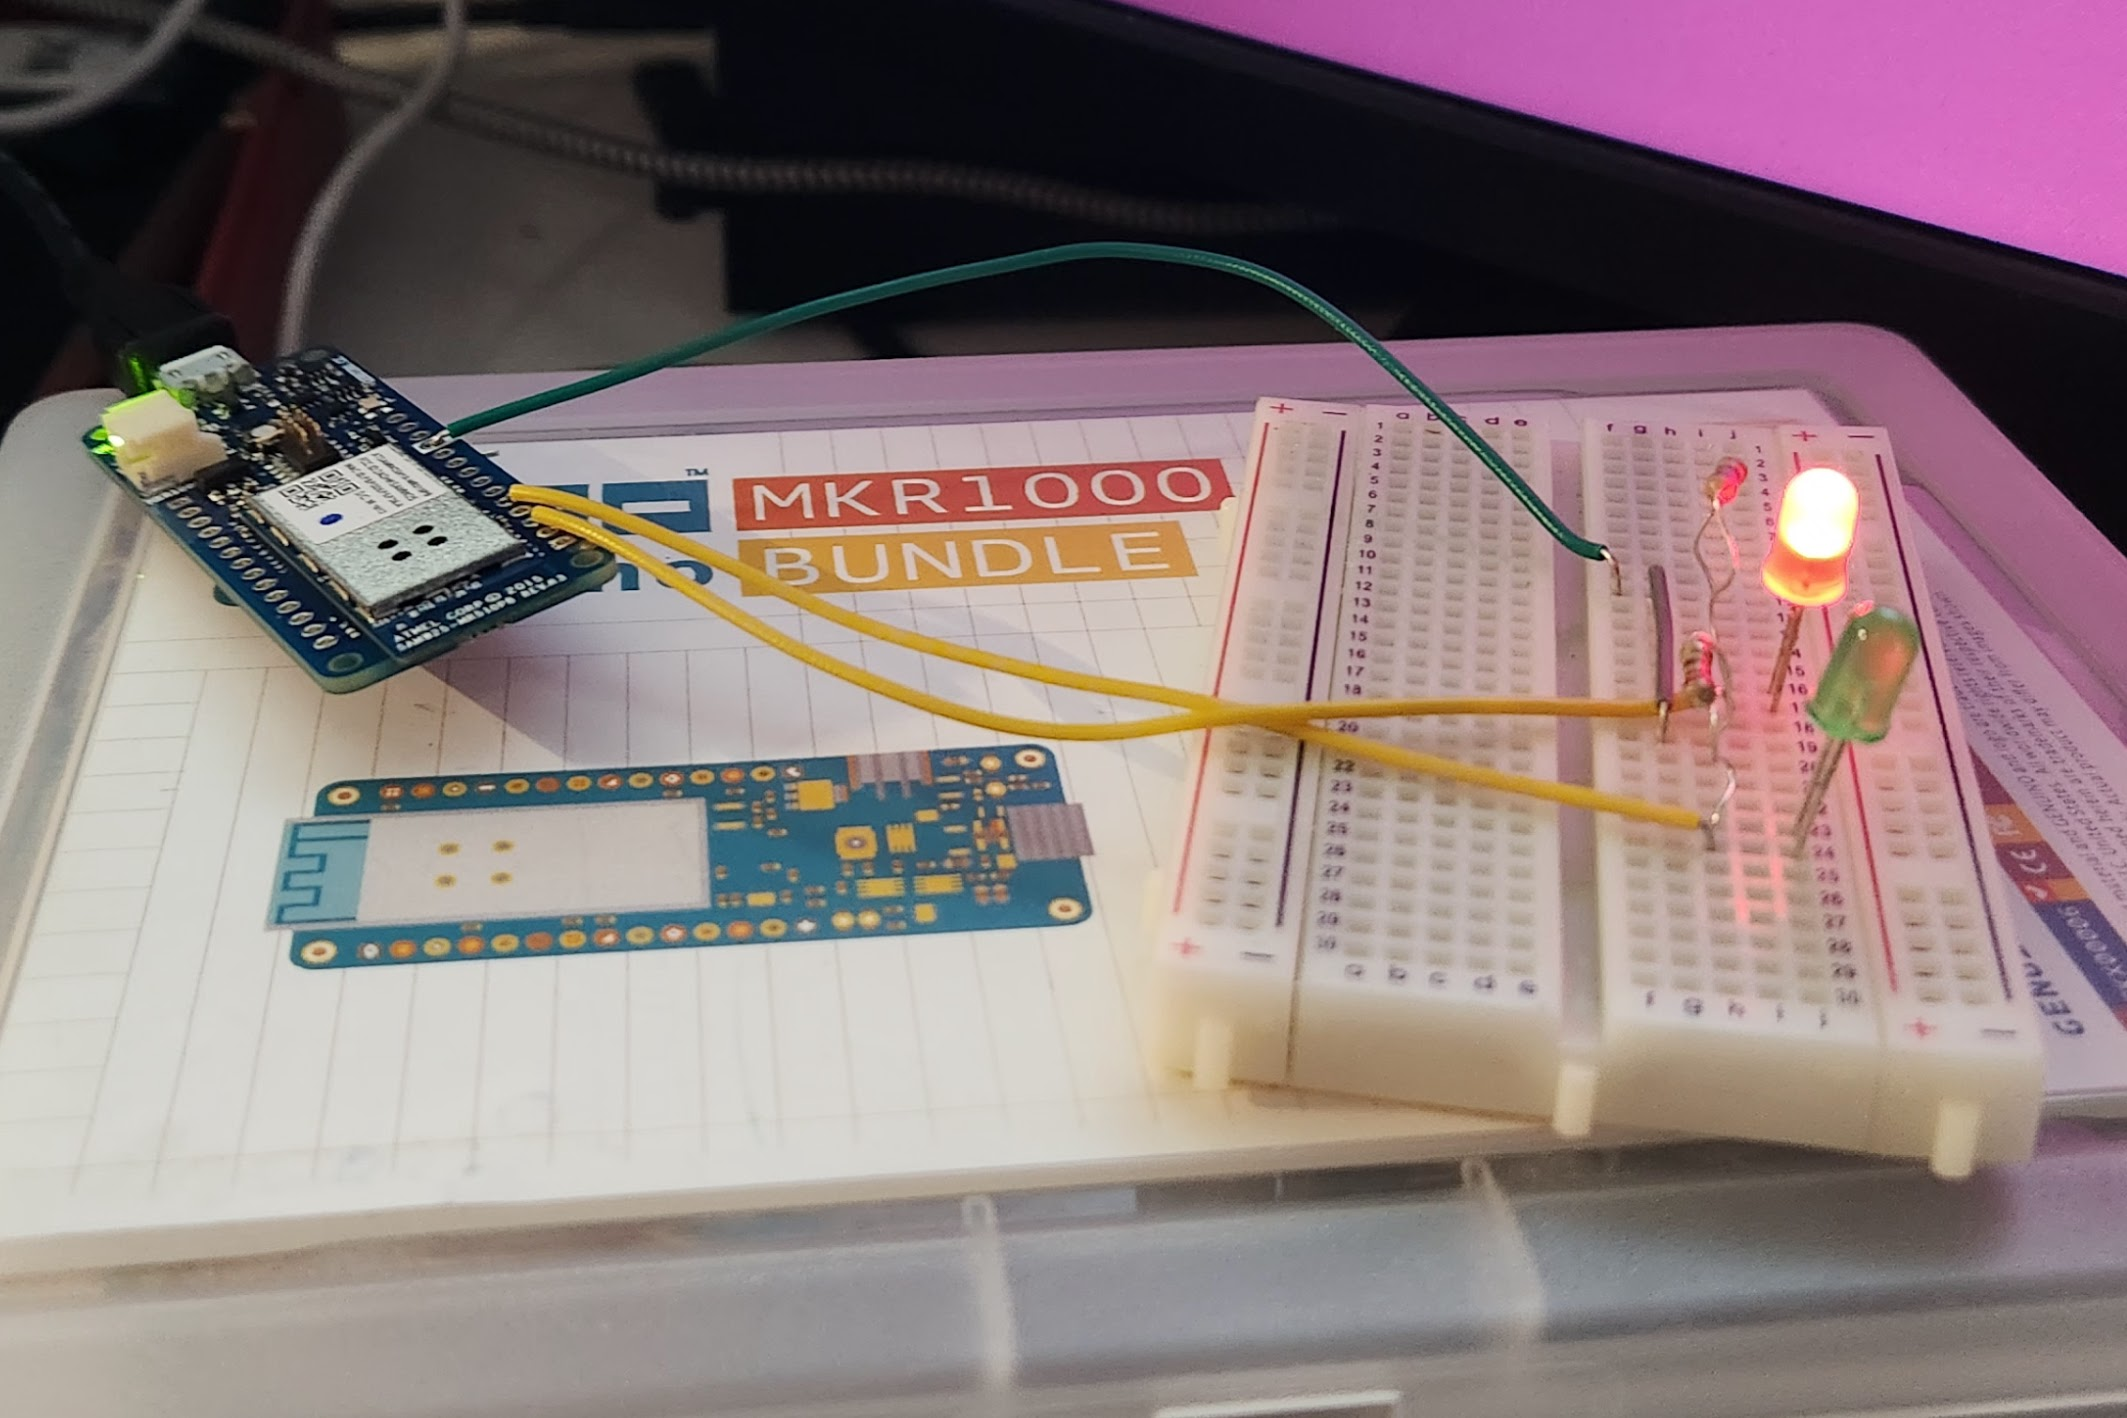
\includegraphics[width=0.99\textwidth]{arduino_btc_project.jpg}
\vspace{8mm}
\end{minipage}
}


\section{More}
{\small

\subsection{Awards}

\cvitem{2014}{ GRE test score: Verbal 165 ($95^\circ$ percentile), Quantitative : 170 ($98^\circ$ percentile), Analytical: 4.0 ($56^\circ$ percentile }
\cvitem{2009}{Italian Olympics of Mathematics: Gold}
\cvitem{2008}{Italian Olympics of Information Technology: Bronze}
\cvitem{2006}{Special mention in high school literary prize ``Le ali dell'Ippogrifo''}

\subsection{Hackatons}

\cvitem{12-13/12/15}{\href{https://www.h-farm.com/en}{H-Farm} H-Ack Luxottica: ideas for the future of glasses. } 
\cvitem{19-20/03/16}{\href{https://www.h-farm.com/en}{H-Farm} H-Ack Food: reinventing the 'Bio food' experience. }
}
\end{document}
